\documentclass[11pt,a4paper]{article}
\usepackage[latin1]{inputenc}
\usepackage{amsmath}
\usepackage{amsfonts}
\usepackage{amssymb}
\usepackage{amsthm}
\usepackage{cite}
\newtheorem{theorem}{Theorem}[section]
\newtheorem{proposition}[theorem]{Proposition}
\newtheorem{definition}[theorem]{Definition}
\newtheorem*{note}{Note}
\usepackage{chngcntr}
\usepackage[ampersand]{easylist}
\usepackage{caption}   
\usepackage{subcaption}
\usepackage[left=2.5cm, right=2.5cm, top=2cm, bottom=2cm]{geometry}
\renewcommand{\baselinestretch}{1.5}
\usepackage[pdftex]{graphicx}

\title{\Large{ADA Project} 
\\ Name: Daitong Li\\ UNI: dl2991
}


\usepackage[pdftex]{graphicx}

\begin{document}
\SweaveOpts{concordance=TRUE}
\maketitle
\newpage

\section*{Cluster Analysis}
The social network analysis in the previous section has discovered close relationship between Clinton and a group of her email receivers. The cluster analysis in this section focuses on classifying the receivers' emails in a meaningful way. It is useful to inspect the trends of the language Clinton has used when speaking with different people/groups of people. The clustering analysis is normally useful to categorize large sum of text into groups based on similarities. For exploratory purpose while analysing Clinton's emails, we would like to see if we can categorize based on the language used emails from different circles of people. Due to time limit, we only focuses on the top 10 accounts who have received most emails from Clinton.

\subsection*{Receivers}
Using the emails datasets, there are 1906 number of people who have received emails from Hillary. We selected 10 receivers who have received highest numbers of emails from Clinton directly.
These receivers are a mix of both work email addresses as well as personal addresses. For example Huma Mahmood Abedin, the vice chair of Hillary Clinton's 2016 presidential campaign, has received 331 emails through her work email address abedinh@state.gov and 31 through personal email. 
The top 10 email receivers are as below:
\begin{center}
  \begin{tabular}{ |l| l | c | c |c|}
    \hline
    &Name & Email Type & Frequency & Word count (cleaned)\\ \hline
    1&Huma Mahmood Abedin & Work & 331 & 981 \\ \hline
    2&Cheryl D. Mills & Work & 297 &16145 \\ \hline
    3&Jacob Jeremiah Sullivan & Work & 288 & 1696\\ \hline
    4&Lauren Jiloty & Work & 223 &1993\\ \hline
    5&Lona Valmoro & Work & 129 &8584\\ \hline
    6&Philippe I. Reines & Personal & 49 &15114\\ \hline
    7&Sidney Stone Blumenthal & Personal & 47 &2068\\ \hline
    8&Cheryl D. Mills & Personal & 35 &1786\\ \hline
    9&Monica R. Hanley & Work & 33 &13190\\ \hline
    10&Huma Mahmood Abedin & Personal & 31&6279 \\
    \hline
  \end{tabular}
\end{center}
\\

The length of emails vary much reladless of the number of emails received. In fact we can already see some patterns from the table above just based on the word count. Clinton sent out more lengthy emails to Sidney Blumenthal (personal), Cheryl Mills (personal) and Monica Hanley (work). It makes sense by considering the their roles and specilizations. 
According to Wikipedia, Blumenthal is a journalist specializing in foreign policy, a former aide to President Bill Clinton and a long-time confidant to Hillary. Mills is a lawyer who previously defended Bill Clinton in the 1999 impeachment trial; and Hanley is Hillary's assistant at the state department.
\\
The table below summarizes the roles or occupations of these 8 key persons:
\begin{center}
 \begin{tabular}{ |l|l| } 
  \hline
   Roles & Names  \\
   \hline
\multirow{Special Assistant} 
& Lauren Jiloty \\ & Lona Valmoro \\ & Monica Hanley  \\ 
\hline
\multirow{Senior Policy Advisor} 
& Philippe Reines \\& Jacob Sullivan \\ 
\hline
\multirow{Political Journalist} 
& Sidney Blumenthal \\ 
\hline
\multirow{Lawyer} & Cheryl Mills \\
\hline
\multirow{Political Staffer} & Huma Abedin \\ 
\hline
\end{tabular}
\end{center}
Huma Abedin recieved highest amount of emails from Hillary, though mainly brief. She served as the Vice Chair for Hillary's 2016 presidential canpaign and was preciously the Deputy Chief of Staff to Secretary of State Hillary Clinton from 2009 to 2013. The two senior advisors also have deep connecitons with Hillary. Jacob Sullivan spoecializes in foreign policy and was the advisor to Hillary during the campaign. Philippe Reines served as the Deputy Assistant Secretary of State for Strategic Communications in 2010 and was a senior advisor to Secretary of State Hillary Clinton in 2009.Other accounts which have received frequent emails from Clinton are Anne-Marie Slaughter, Richard Verma, Robert Russo, Lissa Muscatine (speech writer) etc. all under 30 emails. 
The word count reflect Hillary's language style already to different people, we would like to carry out the cluster analysis in terms of text similarities to answer quesiton like: 
\begin{enumerate}
  \item Does Hillary talk about similar key issues to certain (group of) people?
  \item can we separate emails sent to private accounts from the emails sent to work accounts, based on language used?
\end{enumerate}



\newpage
\subsection*{Emails} 
First we cleaned and transformed the text by 
\begin{enumerate}
\item Convert into lower case. Remove problematic symbols, punctuations and numbers.
\item Remove stop words including 'date', 'can', 'we', 'will' etc. Remove words that are typical in the emails including 'message','sent','original' etc and receivers' names.
\begin{itemize}
\item The cleaned text like "... president nightmare scenarios panetta persuaded renditions tool worth keeping rendition program began carefully monitored form clinton administration bush years transformed ..."
\end{itemize}
\item Convert all documents into a document-term matrix
\begin{itemize} 
\item The matrix has 10 rows representing each email receiver's account; and 20792 columns representing unique words that have appeared in all the email text
\item In each row, if a certain word appears N times the corresponding column would have 'N' , '0' if not. The sparsity of the matrix is 74\%, the non-/sparse entries are 53249/155201. 
\end{itemize}
\item Compute Euclidean distance between each documents.
\end{enumerate}
The distance between documents is defined in 20792 dimensional space. To illustrate for instance, if we have two documents Doc1 (house,libya, document) and Doc 2 (house, information, release, document). In the document-term matrix, the two documents is represented by word frequency eg. we can have Doc1=(1, 0, 1, 1), Doc2=(1, 1, 2, 1), the distance between Doc1 and Doc 2 will hence be $\sqrt{(1-1)^{2} + (0-1)^{2} + (1-2)^{2} + (1-1)^{2}} = \sqrt{2}$.
A simple word cloud for all 10 documents can be seen below:
\begin{figure}[h!]
    \centering
    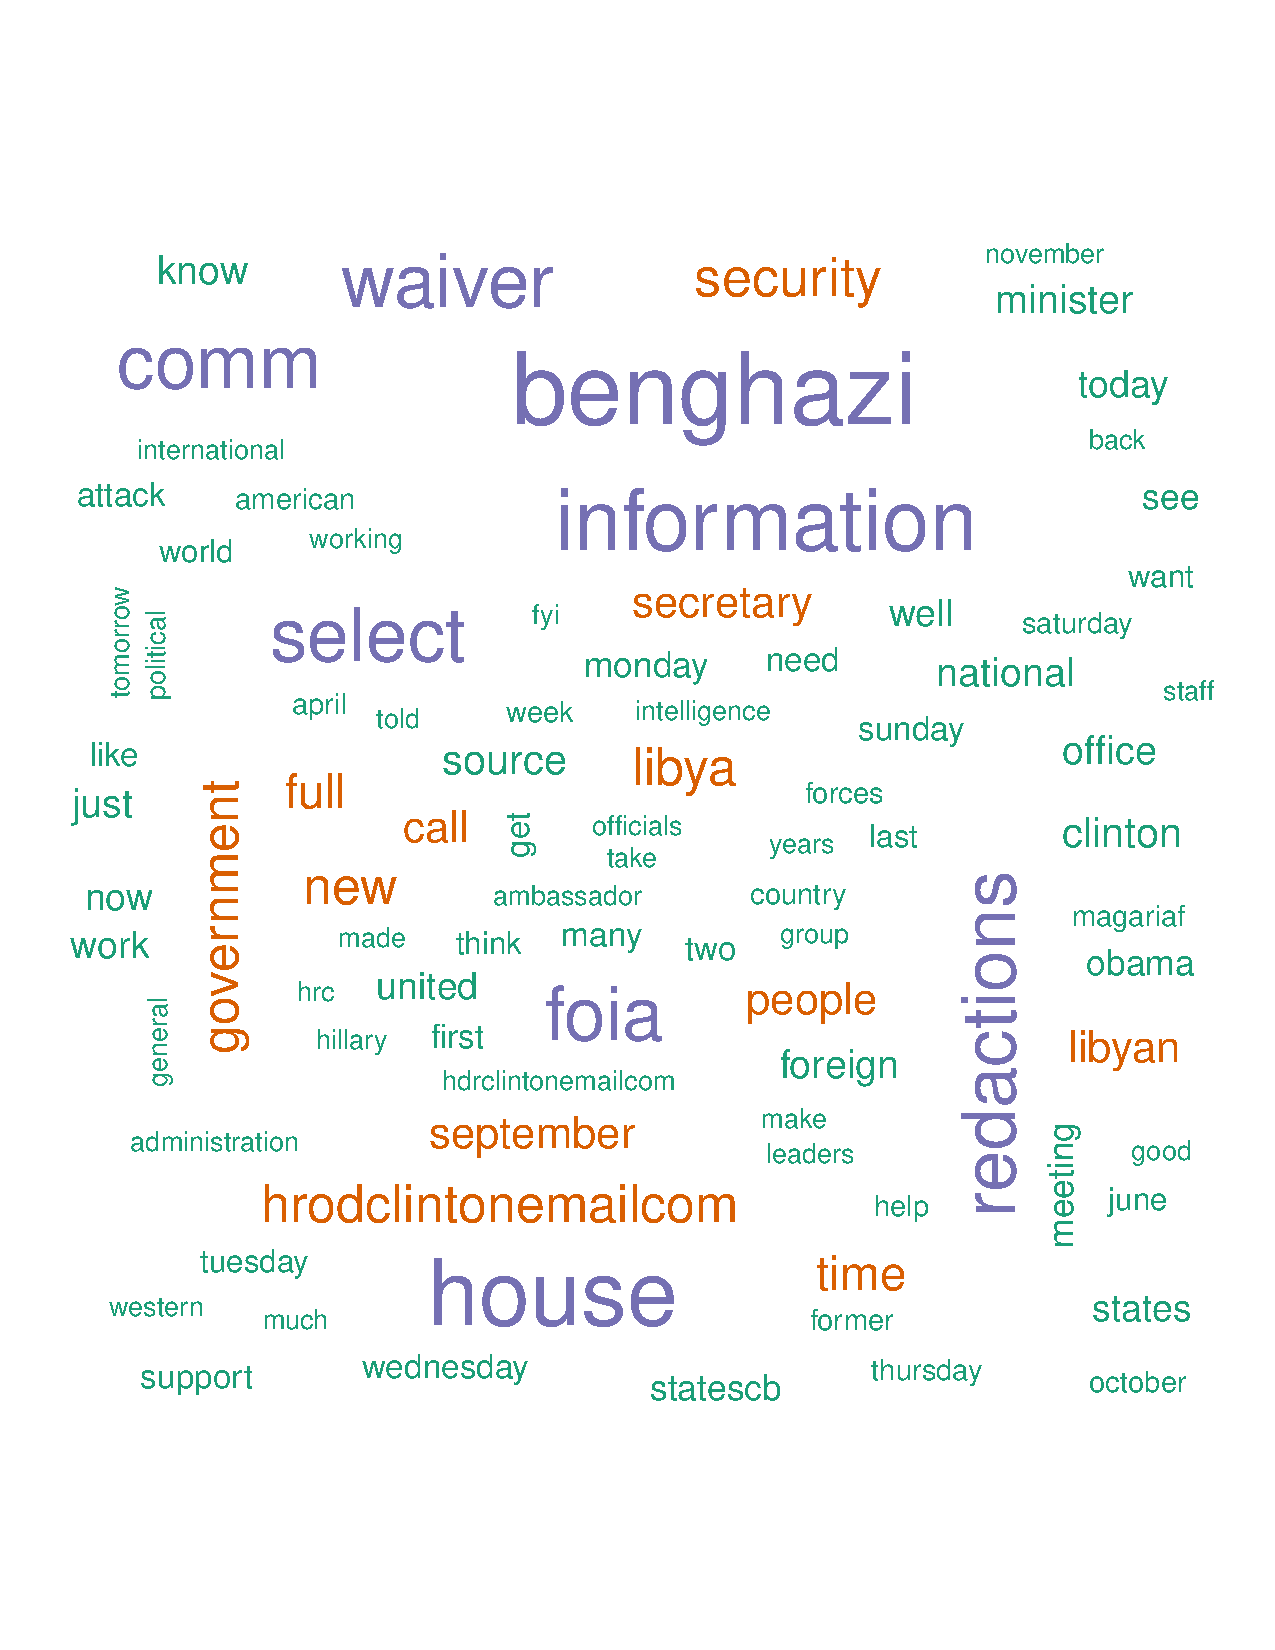
\includegraphics[width=9cm,height=6cm]
    {wcloud.pdf}
    \caption{Word Cloud of Emails}
\end{figure}

\newpage
\subsection*{Clustering Results}
After obtaining the matrix containing the distances between each documents, we tried two methods: hierarchical clustering and K-means. 
\\
For hierarchical clustering, we have used ward.D method or the Ward's minimum variance method. Figure 2 is a cluster dendrogram of the top 10 email accounts. The different colours represents the grouping. The height represents the distance between each document. For example, at distance of 800 we can separate the group in pink and others. The calculation of distance is explained in the section above.
\begin{figure}[h!]
    \centering
    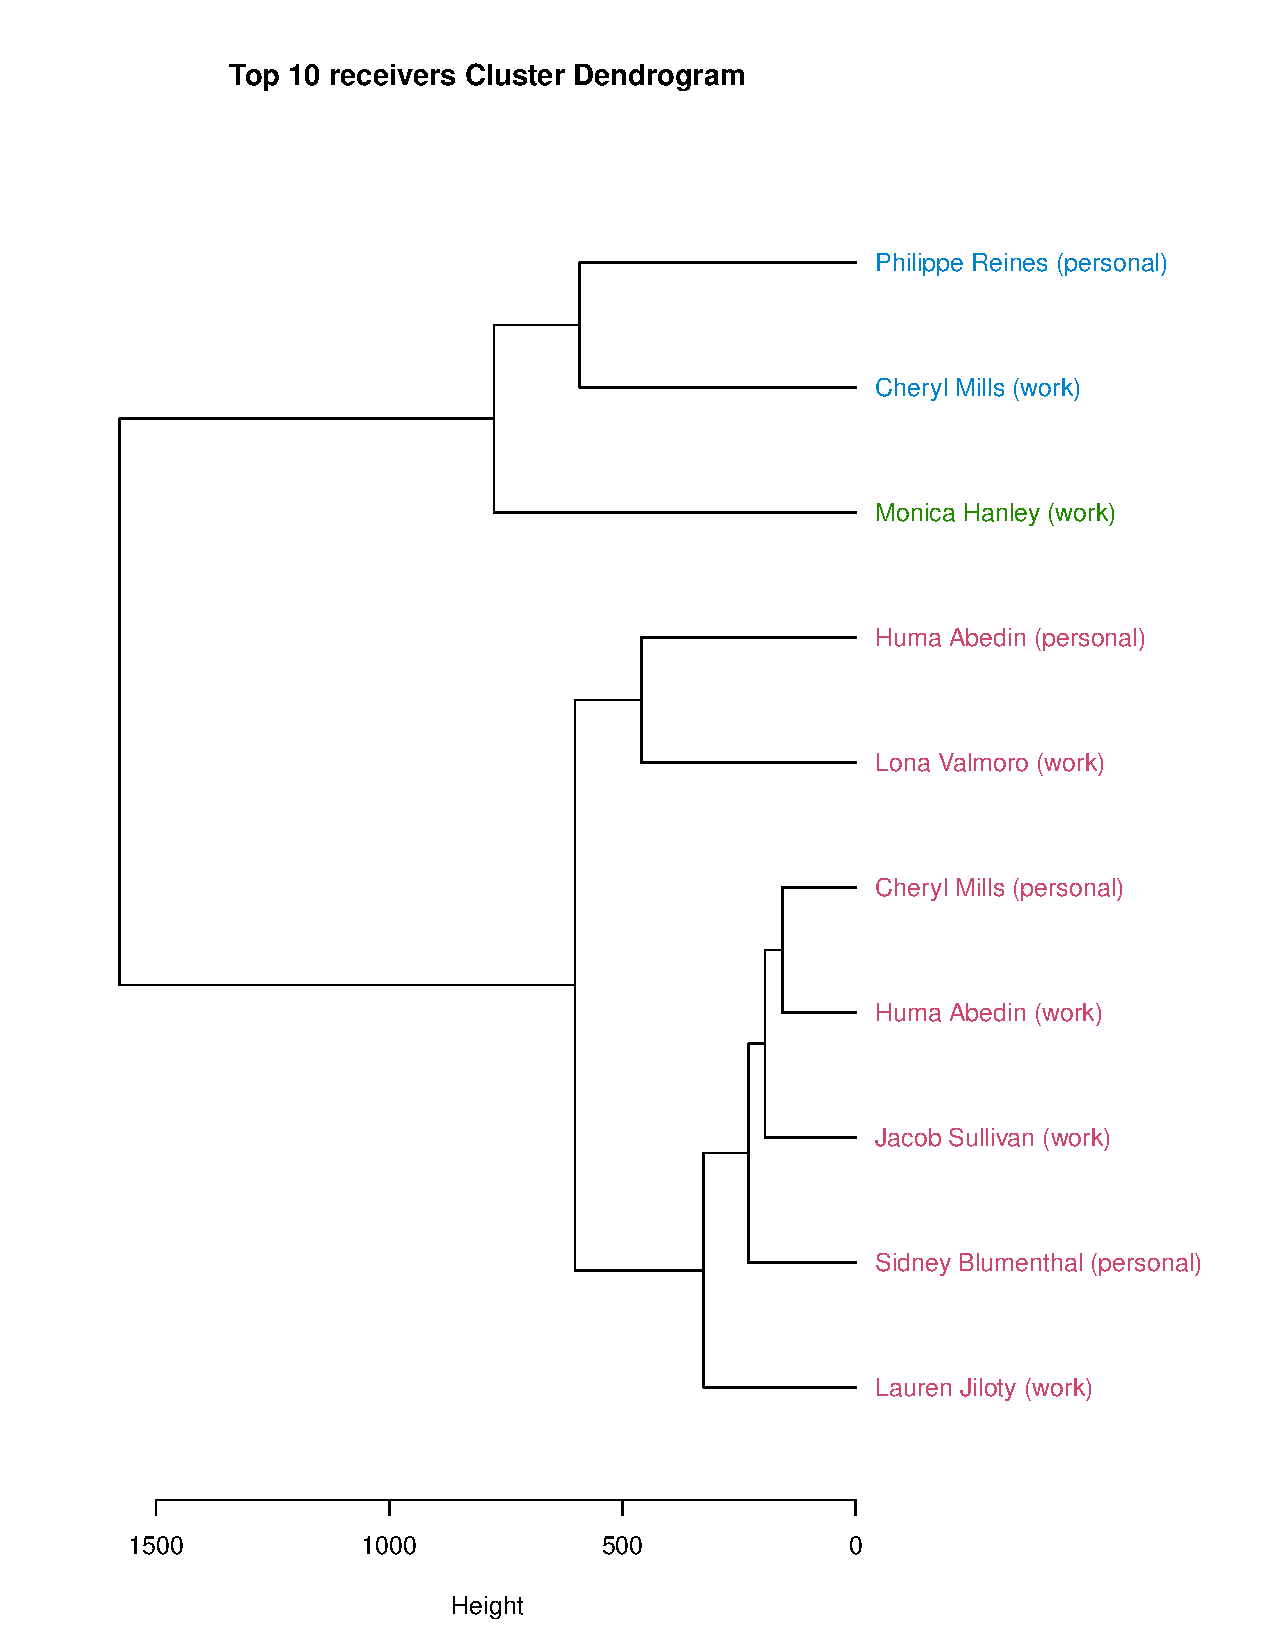
\includegraphics[width=10cm,height=10cm]
    {clusterp.pdf}
    \caption{Dendrogram of top 10 receiver accounts}
\end{figure}

We can also use K-means to determine the clusters. By plotting the within group sum of square versus K, we can see that K=2 or K=3 might be appropriete group numbers for this dataset.

The cluster plots with K=2 and K=3 can be shown in Figure 3 and 4 below. The x and y axis are represented by the first and second component from the PCA analysis. As we can see that the first two components explain more than 95\% of the variance, allowing the clusters to be well separated. 
\\
The results of K-means agree with the results from hierachical clustering. With K=2, we have Sidney Blumenthal (personal), Cheryl Mills (personal) and Monica Hanley (work) in one group (call it Cluster 1) and other accounts in the second group. With K=3, we have Sidney Blumenthal (personal), Cheryl Mills (personal) in group one, Monica Hanley (work) in group two and other accounts in group 3.

\begin{figure}[h!]
    \centering
    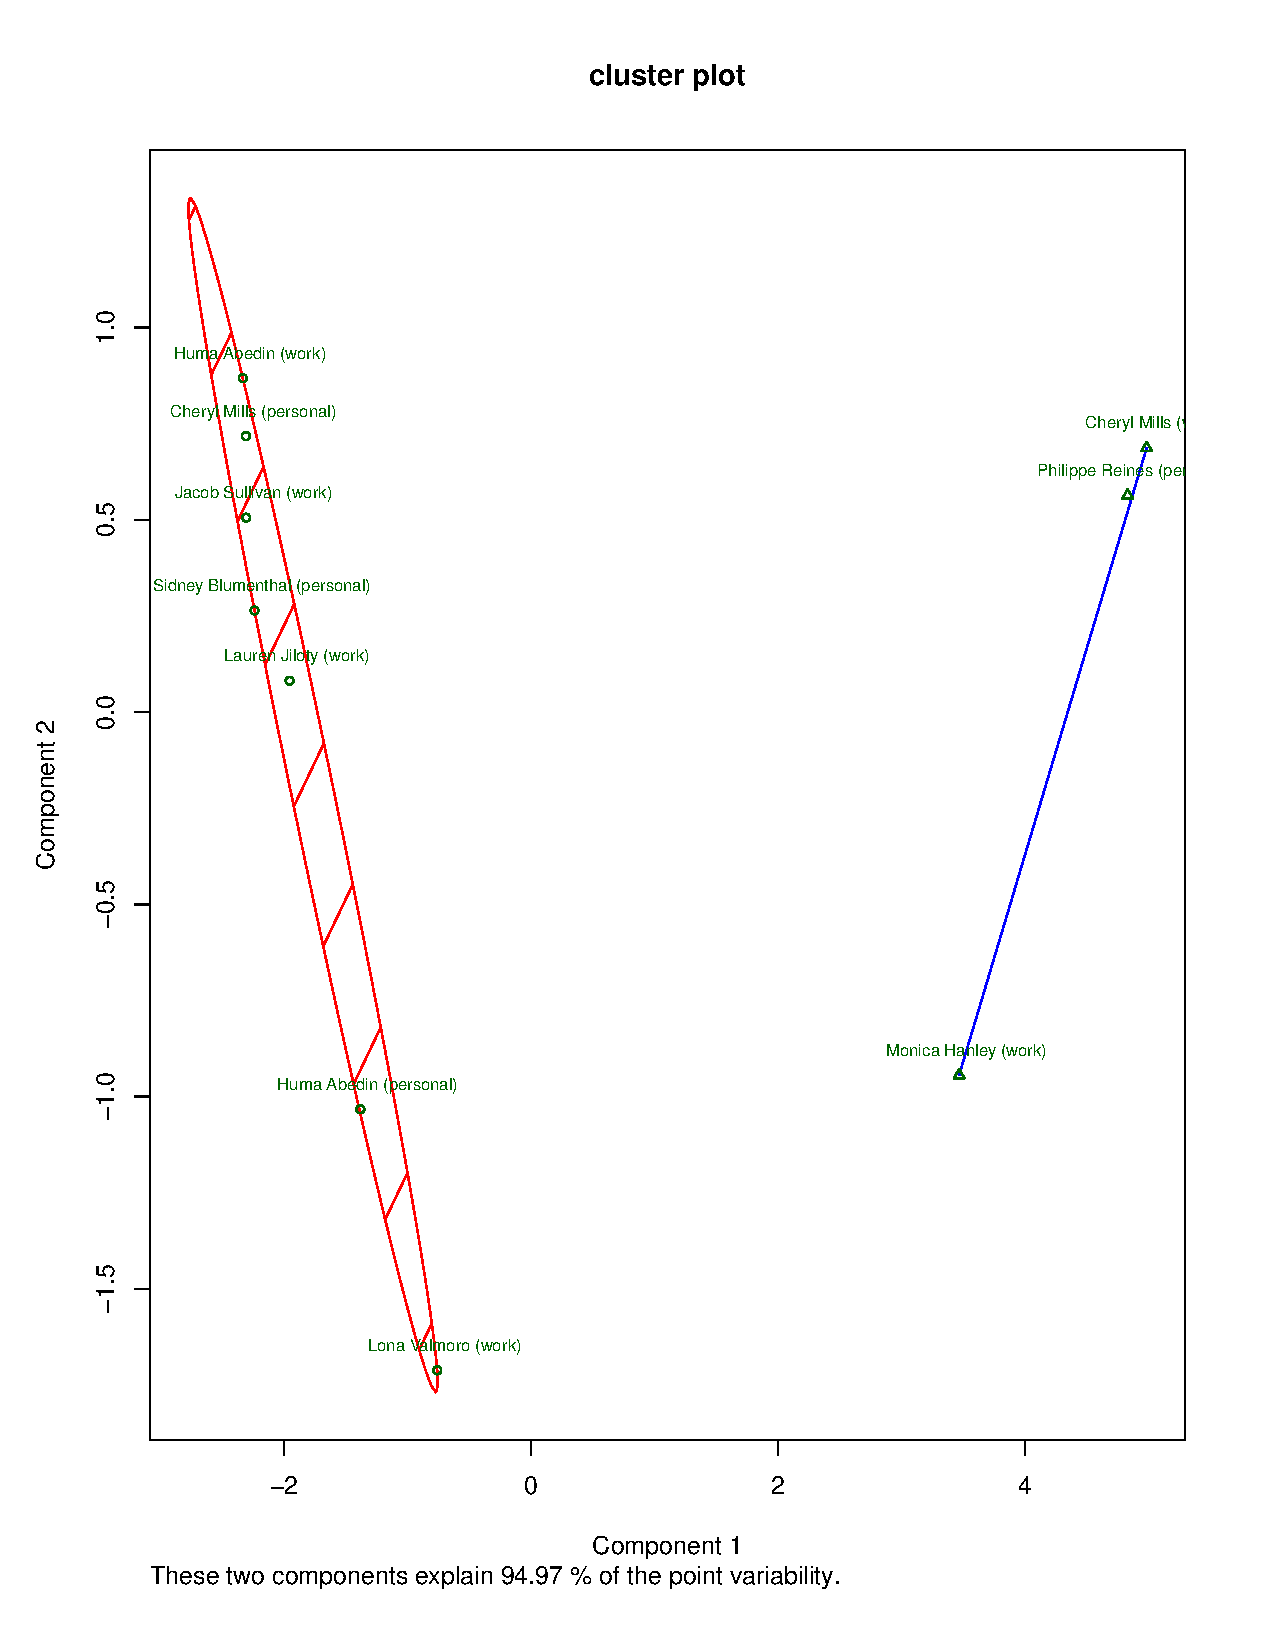
\includegraphics[width=10cm,height=9cm]
    {c2.pdf}
    \caption{Cluster Plot with K=2}
\end{figure}

\begin{figure}[h!]
    \centering
    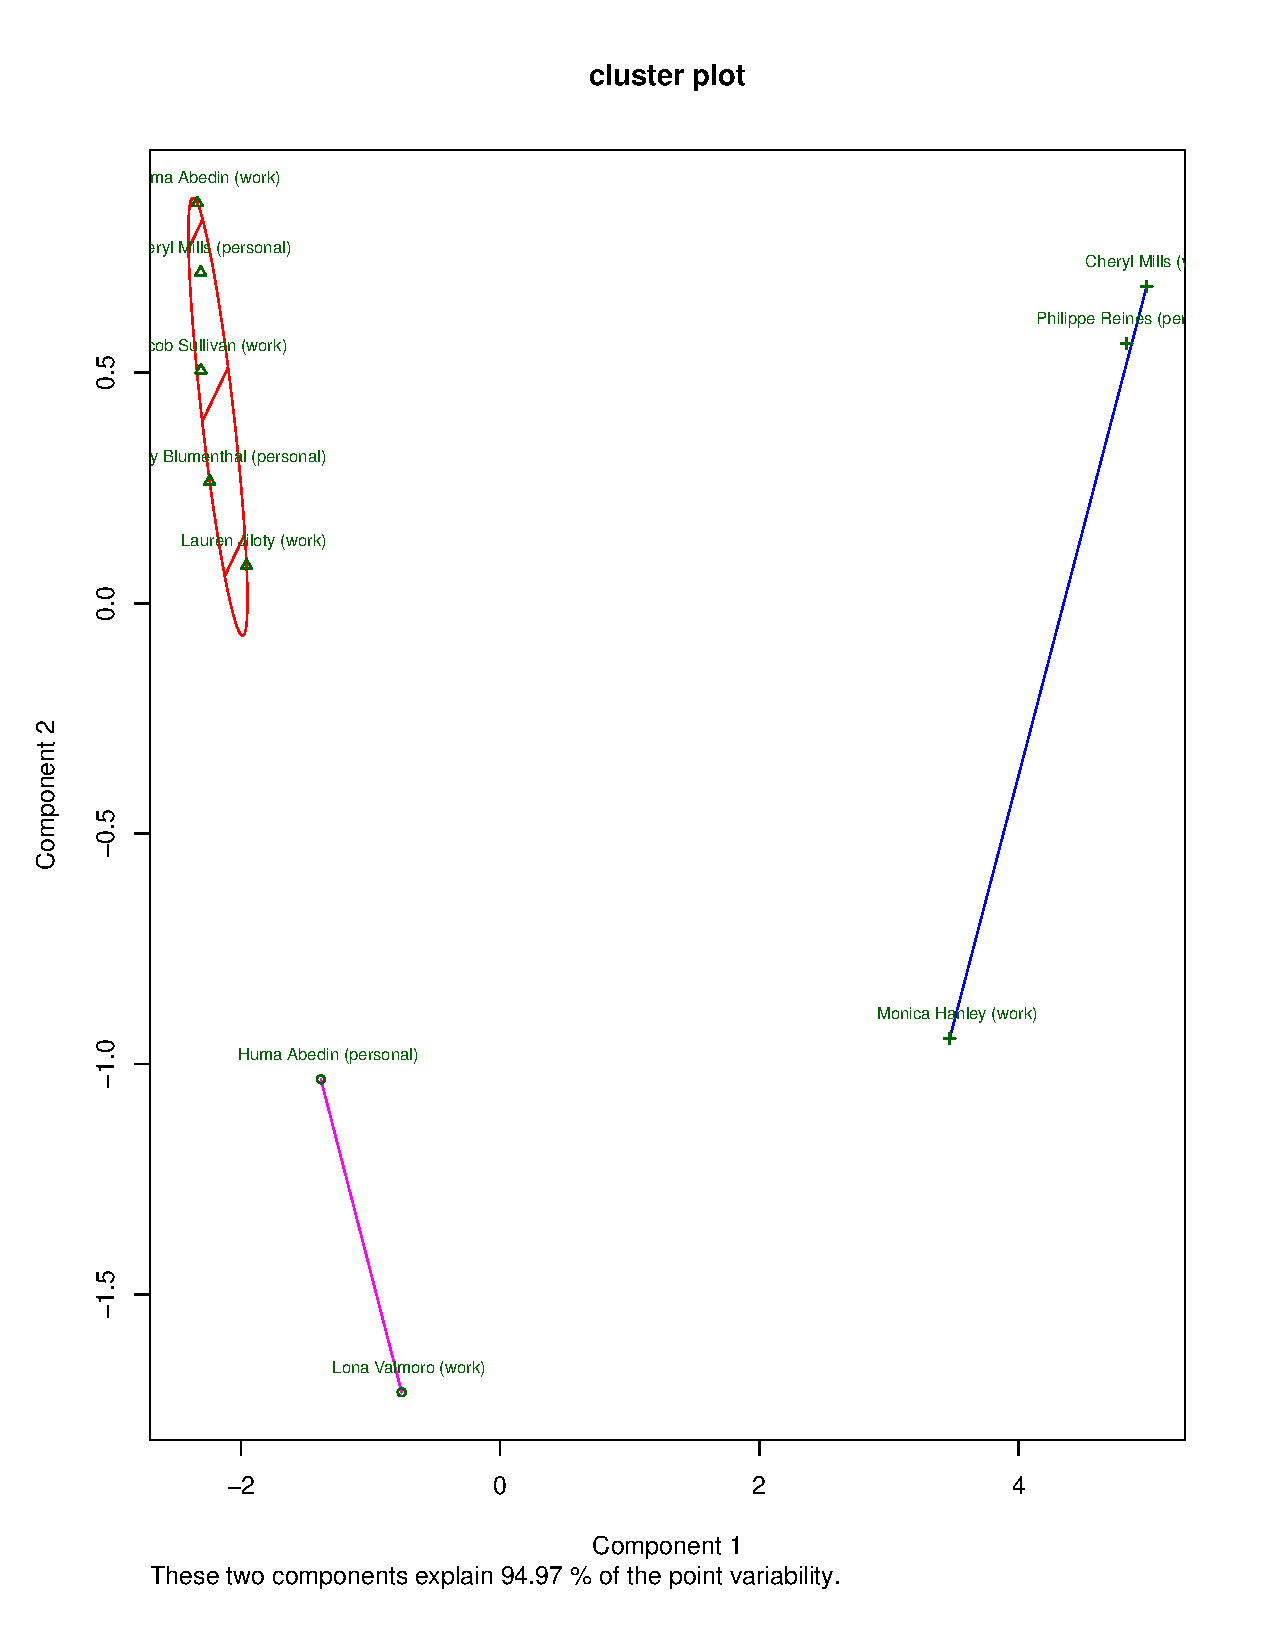
\includegraphics[width=10cm,height=9cm]
    {c3.pdf}
    \caption{Cluster Plot with K=3}
\end{figure}

\newpage
Further more, we can inspect the most frequent words mentioned by Clinton to each cluster of receivers. Below is the top 5 words used by each of the two clusters. Both clusters share common words like Benghazi, sensitive and house; though Hillary talked about the term 'agreement' more with the journalist and the lawyer; and the term 'release' more with her aides and advisors. 
\\

\begin{center}
\begin{tabular}{ |p{3cm}|p{3cm}|| p{3cm}|p{3cm}|  }
 \hline
 \multicolumn{4}{|c|}{Top 5 Most Frequent Words} \\
 \hline
 Words (Cluster 1)  & Percentage of Occurance & Words (Cluster 2) & Percentage of Occurance\\
 \hline
 benghazi & 0.76\% & release  & 0.701\% \\
 house &  0.68\% & benghazi & 0.56\% \\
 sensitive & 0.65\% & house & 0.53\%\\
 information & 0.63\% & information & 0.47\%\\
 agreement & 0.57\% &  sensitive  & 0.46\% \\
 \hline
\end{tabular}
\end{center}

\newpage
\subsection*{Conclusion and Limitations}
The style of language in Hillary's emails to her closely connected lawers and journalist is more much more lengthy and more concentrated in discussing certain 'agreement' terms. In fact, 50\% of all texts of Hillary's emails are contributed to Sidney Blumenthal and Cheryl Mills, among the top 10 receivers. Hillary also talks in similar lengthy style with her aide Monica Hanley. These three receivers are cluster into one group, by analyzing the text similarities. 
\\
This grouping, however, might also cased by the availability of data. If we had more emails of the other receivers, the clustering results might be different. Another limitation is the number of receivers concerned. Due to time limit, only 10 receivers are considered, this might have limited the analysis to certain language style for the top receivers. Moreover, most of the emails in this dataset are partial. The full email text might reveal new characteristics of the language style and thus leads to different clustering. \\
Hence the future work might be with better dataset, to analyze more receivers, with more complete email text and different clustering methods.



\end{document}
